% !TEX TS-program = pdflatex
% !TEX encoding = UTF-8 Unicode

% This is a simple template for a LaTeX document using the "article" class.
% See "book", "report", "letter" for other types of document.

\documentclass[11pt]{article} % use larger type; default would be 10pt

\usepackage[utf8]{inputenc} % set input encoding (not needed with XeLaTeX)
\usepackage{graphicx}
\usepackage{subcaption}
\graphicspath{{./images/}}

%%% Examples of Article customizations
% These packages are optional, depending whether you want the features they provide.
% See the LaTeX Companion or other references for full information.

%%% PAGE DIMENSIONS
\usepackage{geometry} % to change the page dimensions
\geometry{a4paper} % or letterpaper (US) or a5paper or....
% \geometry{margin=2in} % for example, change the margins to 2 inches all round
% \geometry{landscape} % set up the page for landscape
%   read geometry.pdf for detailed page layout information

\usepackage{graphicx} % support the \includegraphics command and options

% \usepackage[parfill]{parskip} % Activate to begin paragraphs with an empty line rather than an indent

%%% PACKAGES
\usepackage{booktabs} % for much better looking tables
\usepackage{array} % for better arrays (eg matrices) in maths
\usepackage{paralist} % very flexible & customisable lists (eg. enumerate/itemize, etc.)
\usepackage{verbatim} % adds environment for commenting out blocks of text & for better verbatim
% These packages are all incorporated in the memoir class to one degree or another...
\usepackage{color}

%%% HEADERS & FOOTERS
\usepackage{fancyhdr} % This should be set AFTER setting up the page geometry
\pagestyle{fancy} % options: empty , plain , fancy
\renewcommand{\headrulewidth}{0pt} % customise the layout...
\lhead{}\chead{}\rhead{}
\lfoot{}\cfoot{\thepage}\rfoot{}

%%% SECTION TITLE APPEARANCE
\usepackage{sectsty}
\allsectionsfont{\sffamily\mdseries\upshape} % (See the fntguide.pdf for font help)
% (This matches ConTeXt defaults)

%%% ToC (table of contents) APPEARANCE
\usepackage[nottoc,notlof,notlot]{tocbibind} % Put the bibliography in the ToC
\usepackage[titles,subfigure]{tocloft} % Alter the style of the Table of Contents
\renewcommand{\cftsecfont}{\rmfamily\mdseries\upshape}
\renewcommand{\cftsecpagefont}{\rmfamily\mdseries\upshape} % No bold!

%%% END Article customizations

%%% The "real" document content comes below...

\title{Design and Evaluation of a Machine Vision System for Identifying Cracked PV Panels}
\author{Jerome Wynne}
%\date{} % Activate to display a given date or no date (if empty),
         % otherwise the current date is printed 

\begin{document}
\maketitle

\section{Problem Description}

This work developed a system for automatically identifying cracks in PV panels from their 2D grayscale computed tomography images. 50 images were provided, of which 38 were deemed to be cracked. Several of these images are shown in Figure \ref{fig:sample_panels}.
\begin{figure}[h!]
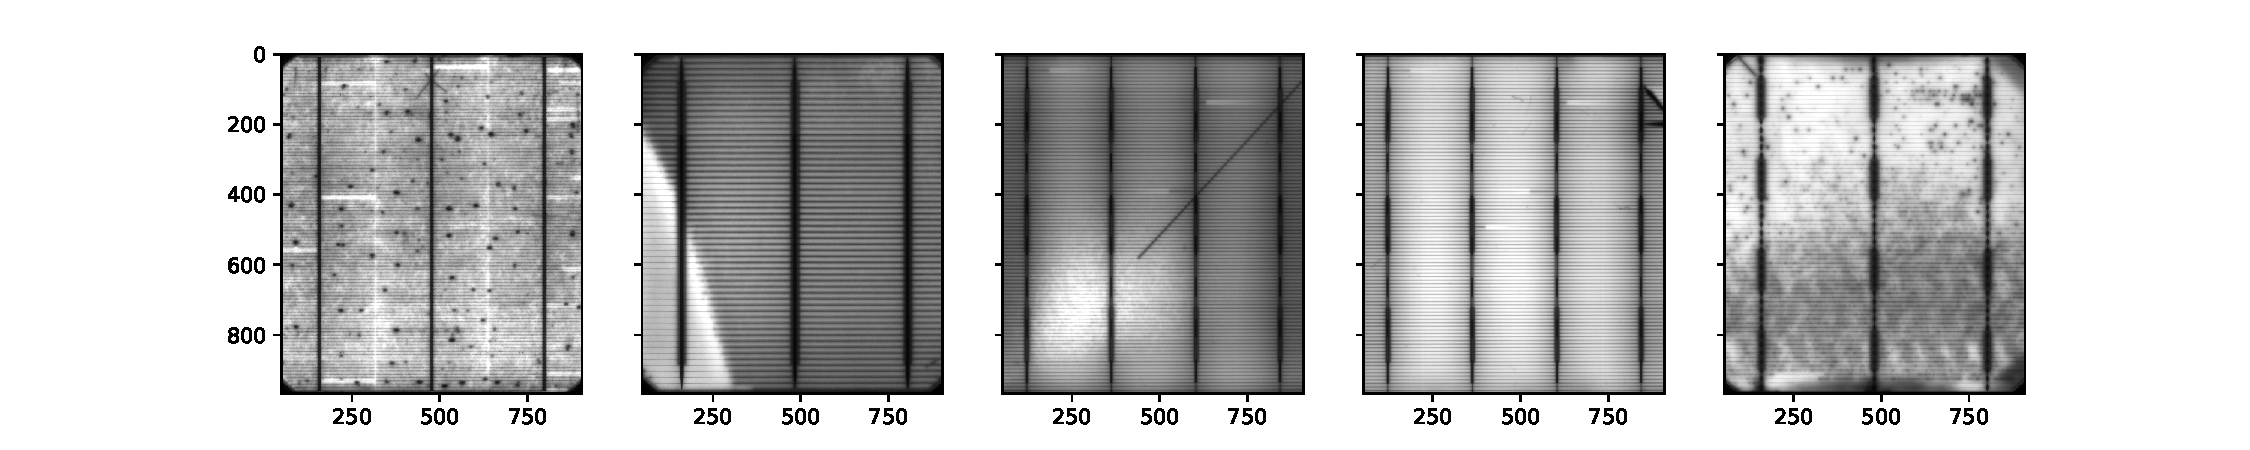
\includegraphics[width=\textwidth]{sample_panels.pdf}
\caption{Scans of the PV panels that were analyzed for damage. The first, third, fourth, and fifth panels from the left contain cracks. Pock-marks similar to those seen on the first panel were not regarded as cracks.}
\label{fig:sample_panels}
\end{figure}

 The median frame height for these images was 965 pixels; their width was similar. Depending on the model and filters used, the images were shrunk for processing.


As can be deduced from Figure \ref{fig:crack_v_scratch}, it was sometimes difficult to ascertain whether a given mark was a crack or a scratch. For the purposes of this work, the latter were considered to be fainter and wigglier - heuristic measures in the absence of any conveniently quantifiable differences. The labels themselves consisted of manually drawn binary masks, an example of which is shown in Figure \ref{fig:mask_example}. Each pixel in a mask was in effect indicators representing whether the associated image pixel was part of a crack. {\color{red}The masks were validated by a panel inspector}. The centers of thick cracks were not labelled on the basis that they would make learning difficult if small kernel sizes were to be used. A 20$\times$20 window centered on a thick crack for example, would be a dark array almost indistinguishable from other dark non-crack regions in the images (in the absence of positional information, at least).

\begin{figure}[h!]
\centering
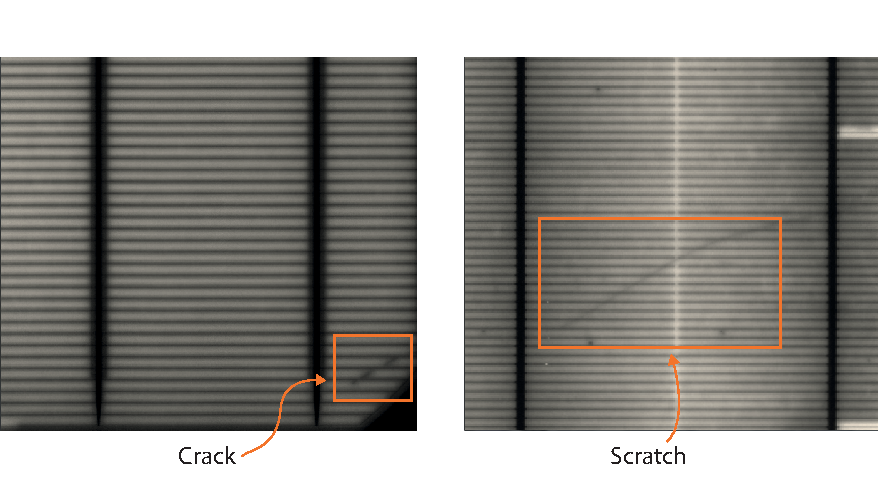
\includegraphics[width=0.7\textwidth]{crack_v_scratch.pdf}
\caption{Distinguishing between cracks and scratches was difficult in certain cases, making ground truth labels somewhat subjective.}
\label{fig:crack_v_scratch}
\end{figure}

Observed sources of noise in the images were as follows:
\begin{itemize}
	\item Dead cells (cells that were unusually bright relative to their neighbors)
	\item Scratches and marks (dark lines)
	\item Debris in the scanner (dark patches)
	\item Hail damage (dark pock-marks)
	\item Variation in the panel model (variation in the panel's layout)
	\item Delamination (low-frequency intensity variation)
\end{itemize}

\begin{figure}[h!]
\centering
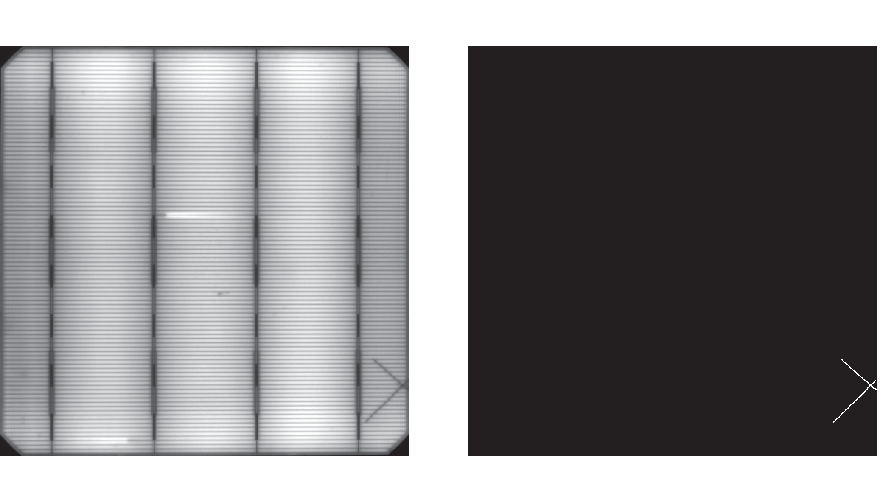
\includegraphics[width=0.7\textwidth]{mask_example.pdf}
\caption{A panel image and its associated set of labels.}
\label{fig:mask_example}
\end{figure}

The ideal panel classifier was defined as being one that:
\begin{itemize}
	\item Provided accurate classification of panels according to the classes cracked/not cracked.
	\item Provided estimates of class membership probabilities to allow operators to tune the model's sensitivity.
	\item Provided per-pixel classification to enable an operator to quickly the area flagged as being cracked.
	\item Operated within reasonable time and compute constraints.
\end{itemize}
Interpretability was not considered a priority.


\subsection{Pre-Processing}
Various filters were applied to the images in an attempt to emphasize cracks and suppress other features. Horizontal differencing of pixel intensities proved to be an effective means of filtering the horizontal cells. A $3\times3$ Laplace filter was used to achieve this effect - a Prewitt filter was also tested, but yielded basically identical results.  A large proportion of the cracks were found to propagate diagonally, an attribute that was exploited by applying a pair of Gabor filters to the image then taking the magnitude of the difference between their real components. The Gabor kernel used is shown in Figure \ref{fig:Gabor_kernel}. By combining horizontal differencing and the described Gabor filtering, the diagonal cracks were substantially enhanced relative to the rest of the image, with the exception of the panel's corners. This process and its results are shown in \ref{fig:filter_process}.

\begin{figure}
\centering
\includegraphics[width = 0.5\textwidth]{Gabor_kernel.pdf}
\caption{The real component of the two Gabor filters applied to the images. The other filter was equivalent but flipped across the vertical axis.}
\label{fig:Gabor_kernel}
\end{figure}

As an alternative method for extracting information pertaining to edge orientation, histograms of oriented gradients were used. An image's gradients were estimated using a combination of Laplace filters, then their magnitudes were accumulated in bins corresponding to distinct orientations. The bin counts in each cell were normalized relative to neighboring cells, then the cell histograms were flattened and concatenated to be fed into classifiers that accepted vector inputs. So far, HOGs have only been tested against classifiers accepting vectors: one possible line of enquiry is to pass them to classifiers accepting tensors of higher orders. Aside from HOGs, the Hough transform may also be a promising candidate for identifying diagonal lines that do not correspond to the panel's corners. It has yet to be trialled.


\subsection{Modeling}
The models trialled so far include:
\begin{itemize}
	\item Generative models against pixel intensity (i.e. modeling local pixel intensities using a multivariate normal distribution)
	\begin{itemize}
		\item These were also tested as filters, the output of which was fed to a nonlinear classifier. An example of this sequence is shown in Figure \ref{fig:normal_then_randomforest}.
	\end{itemize}
	\item Canned classifiers from \texttt{sklearn} - random forest, radial-basis function support vector machines, logistic regression.
	\item Shallow convolutional neural networks against pixel intensity.
\end{itemize}

\begin{figure}[h!]
\includegraphics[width=\textwidth]{normal_then_randomforest.pdf}
\caption{Left: raw image. Center: Log-odds returned by a normal model fit to 20$\times$20 patches of cracks. Right: Crack probabilities returned by a random forest fit to the log-odds returned by the normal model. (This needs a colorbar!)}
\label{fig:normal_then_randomforest}
\end{figure} 

TBC

\begin{figure}
\centering
  	 \begin{subfigure}[b]{1\textwidth}
   	\includegraphics[width=\textwidth]{demo_images.pdf}
   	\caption{Raw images.}
   	\label{fig:b} 
	\end{subfigure}

  	 \begin{subfigure}[b]{1\textwidth}
   	\includegraphics[width=\textwidth]{sobelv.pdf}
   	\caption{Vertical Sobel filter.}
   	\label{fig:b} 
	\end{subfigure}
	
  	 \begin{subfigure}[b]{1\textwidth}
   	\includegraphics[width=\textwidth]{sobelv_gaborne.pdf}
   	\caption{Vertical Sobel filtering followed by a Gabor filter.}
   	\label{fig:d} 
	\end{subfigure}
	
	
  	 \begin{subfigure}[b]{1\textwidth}
   	\includegraphics[width=\textwidth]{sobelv_gabordiff.pdf}
   	\caption{Vertical Sobel filtering followed by a difference of two Gabor-filtered images.}
   	\label{fig:f} 
	\end{subfigure}
	
	\begin{subfigure}[b]{1\textwidth}
   	\includegraphics[width=\textwidth]{demo_masks.pdf}
   	\caption{Original image masks (i.e. ground truth).}
   	\label{fig:f} 
	\end{subfigure}
\caption{}
\label{fig:filter_process}
\end{figure}


\end{document}
